% THIS IS SIGPROC-SP.TEX - VERSION 3.0
% WORKS WITH V3.1SP OF ACM_PROC_ARTICLE-SP.CLS
% JUNE 2007
%
% It is an example file showing how to use the 'acm_proc_article-sp.cls' V3.1SP
% LaTeX2e document class file for Conference Proceedings submissions.
% ----------------------------------------------------------------------------------------------------------------
% This .tex file (and associated .cls V3.1SP) *DOES NOT* produce:
%       1) The Permission Statement
%       2) The Conference (location) Info information
%       3) The Copyright Line with ACM data
%       4) Page numbering
% ---------------------------------------------------------------------------------------------------------------
% It is an example which *does* use the .bib file (from which the .bbl file
% is produced).
% REMEMBER HOWEVER: After having produced the .bbl file,
% and prior to final submission,
% you need to 'insert'  your .bbl file into your source .tex file so as to provide
% ONE 'self-contained' source file.
%
% Questions regarding SIGS should be to
% Adrienne Griscti ---> griscti@acm.org
%
% Questions/suggestions regarding the guidelines, .tex and .cls files, etc. to
% Gerald Murray ---> murray@acm.org
%
% For tracking purposes - this is V3.0SP - JUNE 2007

\documentclass{sig-alternate}

\include{macros}

\begin{document}

\title{Automated Method Sequence Generation for Structural Test Generation}
%
% You need the command \numberofauthors to handle the 'placement
% and alignment' of the authors beneath the title.
%
% For aesthetic reasons, we recommend 'three authors at a time'
% i.e. three 'name/affiliation blocks' be placed beneath the title.
%
% NOTE: You are NOT restricted in how many 'rows' of
% "name/affiliations" may appear. We just ask that you restrict
% the number of 'columns' to three.
%
% Because of the available 'opening page real-estate'
% we ask you to refrain from putting more than six authors
% (two rows with three columns) beneath the article title.
% More than six makes the first-page appear very cluttered indeed.
%
% Use the \alignauthor commands to handle the names
% and affiliations for an 'aesthetic maximum' of six authors.
% Add names, affiliations, addresses for
% the seventh etc. author(s) as the argument for the
% \additionalauthors command.
% These 'additional authors' will be output/set for you
% without further effort on your part as the last section in
% the body of your article BEFORE References or any Appendices.

%\numberofauthors{1} %  in this sample file, there are a *total*
% of EIGHT authors. SIX appear on the 'first-page' (for formatting
% reasons) and the remaining two appear in the \additionalauthors section.
%

%\author{Suresh Thummalapenta$^1$, Tao Xie$^1$, Nikolai Tillmann$^2$, Jonathan de Halleux$^2$, Wolfram Schulte$^2$\\
%\small{$^1$Department of Computer Science, North Carolina State University, Raleigh}\\
%\small{$^2$Microsoft Research, One Microsoft Way, Redmond}\\
%\small{$^1$\{sthumma, txie\}@ncsu.edu, $^2$\{nikolait, jhalleux, schulte\}@microsoft.com}\\
%}

%\author{
% You can go ahead and credit any number of authors here,
% e.g. one 'row of three' or two rows (consisting of one row of three
% and a second row of one, two or three).
%
% The command \alignauthor (no curly braces needed) should
% precede each author name, affiliation/snail-mail address and
% e-mail address. Additionally, tag each line of
% affiliation/address with \affaddr, and tag the
% e-mail address with \email.
%
% 1st. author
%\alignauthor
%Suresh Thummalapenta\\
%       \affaddr{Department of Computer Science}\\
%       \affaddr{North Carolina State University}\\
%       \affaddr{Raleigh, USA}\\
%       \email{sthumma@ncsu.edu}
%% 2nd. author
%\alignauthor
%Tao Xie\\
%			 \affaddr{Department of Computer Science}\\
%       \affaddr{North Carolina State University}\\
%       \affaddr{Raleigh, USA}\\
%       \email{xie@csc.ncsu.edu}% 3rd. author
%\and
%\alignauthor Nikolai Tillmann, Jonathan de Halleux, Wolfram Schulte\\
%       \affaddr{Microsoft Research}\\
%       \affaddr{One Microsoft Way, Redmond, USA}\\
%       \email{\{nikolait, jhalleux, schulte\}@microsoft.com}  
%}

\maketitle
%\begin{abstract}
%\end{abstract}

%\section{Introduction}

\label{sec:introduction}

Access control is one of the most fundamental and widely used
security mechanisms. It controls which principals (users, processes,
etc.) have access to which resources in a system. To better manage
access control, systems often explicitly specify access control
policies using policy languages such as XACML~\cite{oasis05:xacml}
and Ponder \cite{damianou01:ponder}. Whenever a principal requests
access to a resource, that request is passed to a software component
called a Policy Decision Point (PDP). PDP evaluates the request
against access control policies, and grants or denies the request
accordingly.

The specification of access control policies is often a challenging
problem. It is common that a system's security is compromised due to
the misconfiguration of access control policies instead of the
failure of cryptographic primitives or protocols. This problem
becomes increasingly severe as software systems become more and more
complex, and are deployed to manage a large amount of sensitive
information and resources that are organized into sophisticated
structures.

Formal verification is an important means to ensuring the correct
specification of access control
policies\Comment{~\cite{jajodia97:logical, sandhu99:arbac}}.
Recently, several tools have been developed to verify XACML access
control policies against user-specified
properties~\cite{hughes04:automated,fisler05:verification,zhang05:evaluating}.
However, it is often beyond the capabilities of these tools to
verify complex access control policies in large-scale information
systems. Furthermore, user-specified properties are often not
available~\cite{fisler05:verification}.

Like in software development, errors in access control policies may
also be discovered through testing. In fact, once access control
policies are specified, they are often tested with some access
requests so that security officers may manually check the PDP's
responses against expected ones~\cite{anderson02:xacml}. However,
current policy testing practice tends to be ad hoc. Although there
exist various coverage criteria~\cite{zhu97:software} for software
programs, there are no criteria or good heuristics to guide
systematic generation of high-quality policy test suites. With an ad
hoc policy testing, it is questionable that high confidence could be
gained on the correctness of access control policies.

This paper presents a first step toward systematic policy testing.
We propose the concept of \Intro{policy coverage} to measure the
quality of policy test suites, which are sets of request-response
pairs. Intuitively, the more policy rules (as well as their
components such as subjects, resources, and conditions) are involved
when evaluating a test suite, the more likely it is to discover
errors in access control policies. We have developed a
coverage-measurement tool to measure the coverage of XACML policies
achieved by a set of access requests. We have also developed a
request-generation tool that randomly generates policy test suites
for a given set of policies.

Although the randomly generated test suites can achieve high policy
coverage, and are effective in detecting a variety of policy
specification errors, it may potentially include a huge number of
requests, which makes it difficult to efficiently inspect and verify
the correctness of responses from the PDP. To mitigate this problem,
we further propose a request reduction technique to significantly
reduce the size of a test suite while maintaining its policy
coverage.

Previous experiments~\cite{rothermel98:empirical} showed that test
reduction based on program code coverage can severely compromise the
fault-detection capabilities of the original test suite. To evaluate
the impact of the proposed request reduction technique on the
quality of policy testing, we conduct an experiment on a set of real
policies with mutation testing~\cite{demillo78:hints}, which is a
specific form of fault injection that consists of creating faulty
versions of a policy by making small syntactic changes. In the
experiment, we compare the fault-detection capabilities of the
reduced set and original set of requests. Our experimental results
show that our coverage-based request reduction technique can
substantially reduce the size of generated requests but incur only
relatively low loss in fault detection capabilities. We also conduct
a study that measures the policy coverage of an XACML conformance
test suite as well as a conference reviewing system's policy. Our
results show that the measurement of policy coverage can effectively
identify uncovered parts of policies. Such results can be used to
guide the development of further test cases, significantly improving
the quality of policy testing.

\Comment{ This paper makes the following main contributions:
\begin{itemize}
\item We propose the concept of policy coverage based on
a general access control model. We further instantiate this
concept in the context of XACML, a widely used and standardized
meta policy language
for expressing domain-specific access control requirements.

\item We develop a coverage-measurement tool for automatically
measuring the coverage for XACML policies achieved by a given set
of requests.

\item We develop a request-generation tool for randomly generating
requests for XACML policies and a request-reduction tool for
greedily selecting a minimal set of requests for achieving the
same policy coverage as the original set of requests.

\item We develop initial mutation operators for XACML policies to
conduct mutation testing. We conduct an experiment on a set of
real policies to compare the effectiveness of the minimal set of
requests with the original set of requests in terms of fault
detection. We also conduct a study on policy coverage of existing
manually generated requests.

\end{itemize}
}

The rest of the paper is organized as follows. Section
\ref{sec:xacml} presents background information on XACML, a widely
used and standardized meta policy language for expressing
domain-specific access control requirements.
Section~\ref{sec:model} proposes the concept of policy testing and
policy coverage based on a general access control model. In
Section~\ref{sec:coverage}, we instantiate the concept of policy
coverage in the context of XACML. We also present the design of a
coverage measurement tool. Sections~\ref{sec:reqgen}
and~\ref{sec:reqreduce} describe the request-generation tool and
our request reduction technique, respectively.
Section~\ref{sec:mutation} presents a set of initial mutation
operators developed for policies. Section~\ref{sec:experiment}
presents the experiment conducted to assess request reduction and
its effect on fault detection capabilities.
Section~\ref{sec:experimentalresults} illustrates the study of
measuring the policy coverage achieved by manually generated
requests. Section~\ref{sec:related} discusses related work and
Section~\ref{sec:conclusion} concludes the paper with future
directions.

















\sloppy

%\section{Example}
\label{sec:example}

\begin{figure*}[t]
\centering
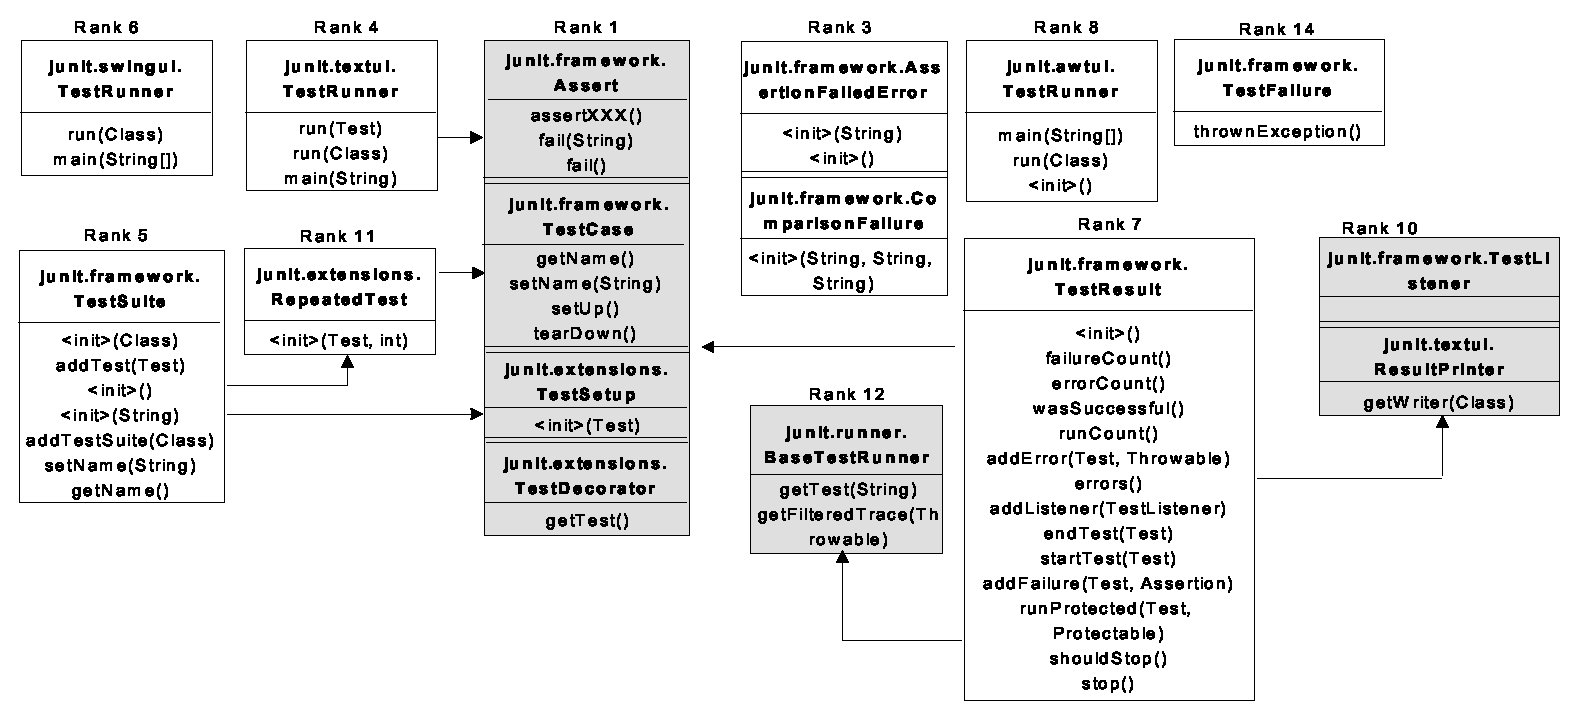
\includegraphics[scale=0.68,clip]{figs/examplehotspot_final.eps}
\caption{Hotspot hierarchies identified for the JUnit framework} \label{fig:hotspotexample}
\end{figure*}

We next use an example to explain our approach and show how the detected
hotspots and coldspots can be used by the framework users. We use JUnit~\cite{JUNIT}, the
\emph{de facto} standard unit testing framework for Java, 
as an illustrative example for explaining our approach.

SpotWeb accepts an input framework, say JUnit, and extracts
\emph{FrameworkInfo} from the framework. The
\emph{FrameworkInfo} includes all classes, all interfaces, public
or protected methods of each class and interface, and inheritance
hierarchy among classes or interfaces of the framework. SpotWeb also captures
the constants defined by the input framework. SpotWeb
constructs different queries for each class or interface and
interacts with a CSE such as Google code search~\cite{GCSE} to
gather relevant code examples from existing open source projects that
reuse the classes of the input framework. For example, SpotWeb constructs
a query such as ``\CodeIn{lang:java junit.framework.TestSuite}'' for
gathering relevant code examples of the \CodeIn{TestSuite} class. These
gathered code examples are referred as a \emph{LocalRepository} for
the input framework. SpotWeb analyzes gathered code examples
statically and computes \emph{UsageMetrics} for classes, interfaces,
and public or protected methods of all classes and interfaces. For
example, the \emph{UsageMetrics} computed for the \CodeIn{TestSuite}
class show that the class is instantiated for 165 times and is
extended for 32 times. Similarly, the \emph{UsageMetrics} computed
for the method \CodeIn{addTest} of the \CodeIn{TestSuite} class show
that the method is invoked for 95 times. SpotWeb also gathers code
examples for each class or method and stores these code examples in
a repository, referred as \emph{ExampleDB}. Then SpotWeb uses the
algorithm shown in Figure~\ref{alg:hotspotalgo} for detecting
hotspots from the computed \emph{UsageMetrics}.

Initially, SpotWeb ranks methods in a non-ascending order based on
their \emph{UsageMetrics} and uses a threshold percentage $HT$ to
detect hotspot methods: the methods in the top $HT$ percentage with
a non-zero \emph{UsageMetrics} are detected as hotspot methods. 
The detected hotspot methods are then
grouped into their declaring classes, detected as hotspot classes.
These hotspot classes are ranked based on the minimum rank of the
hotspot methods declared by these classes. SpotWeb classifies the
hotspot classes into two categories (templates and hooks) based on
heuristics described in Step 4 of the algorithm shown in Figure~\ref{alg:hotspotalgo}. The hotspot classes of each
category are further grouped into hierarchies based on their
inheritance relationships. For example, SpotWeb detected classes
\CodeIn{Assert} and \CodeIn{TestCase} as hook hotspots in the JUnit
framework. As \CodeIn{TestCase} class extends \CodeIn{Assert} class,
SpotWeb groups both the classes into the same hierarchy. SpotWeb
assigns a rank to each hierarchy based on the minimum rank of the
hotspot classes contained in the hierarchy. For example, consider
that the \CodeIn{Assert} class has Rank 1 and the \CodeIn{TestCase}
class has Rank 2, then the grouped hierarchy of the
\CodeIn{Assert} and \CodeIn{TestCase} classes is assigned with Rank
1. The rank attribute uniquely identifies a hierarchy among all
other hierarchies. Hierarchies with smaller ranks have higher preference
or importance to the hierarchies with larger ranks.

Figure~\ref{fig:hotspotexample} shows the hotspot hierarchies detected for the JUnit
framework. The figure also shows ranks assigned to each hierarchy.
As the rank attribute uniquely identifies a hierarchy, we use the
rank as an identity for describing a hierarchy.
Each hierarchy includes one or more hotspot classes and is shown as pairs of class and its methods.
For example, Hierarchy 1 (hierarchy with Rank 1) has classes \CodeIn{Assert}, \CodeIn{TestCase}, \CodeIn{TestSetup},
and \CodeIn{TestDecorator}. We show template hierarchies in white and hook hierarchies in gray.
For example, Hierarchy 1 is a hook hierarchy and Hierarchy 3 is a template hierarchy.

Methods inside each class of a hierarchy are sorted
based on their computed \emph{UsageMetrics}. Sorting methods of a class
can assist the framework users in quickly identifying the methods that are often
used inside a given hotspot class. For example, consider the \CodeIn{TestSuite} class
shown in Hierarchy 5. The \CodeIn{TestSuite} class has three constructors \CodeIn{<init>(Class)},
\CodeIn{<init>()}, and \CodeIn{<init>(String)}. However, the \CodeIn{<init>(Class)} constructor
is often used compared to the other two constructors. Due to space limit,
we show all assertion methods such as \CodeIn{assertEquals} and \CodeIn{assertTrue}
of the class \CodeIn{Assert} of Hierarchy 1 as \CodeIn{assertXXX}.

The figure also displays dependencies among hotspot hierarchies
(shown as arrows between hierarchies). SpotWeb captures the
usage relationships among hotspot classes through dependencies.
For example, Hierarchy $5$ has a
\CodeIn{TEMPLATE\_HOOK} dependency with Hierarchy $1$. This
dependency indicates that to reuse methods such as \CodeIn{addTest}
of the class \CodeIn{TestSuite} in Hierarchy 5, the user has to
define a new behavior for the classes in Hierarchy $1$.

\begin{figure}[t]
\begin{CodeOut}
\begin{alltt}
01:public class SRDAOTestCase 
02:\hspace*{0.4in}extends TestCase \{
03:\hspace*{0.1in}private SRDAO dao = null;...
04:\hspace*{0.1in}public SRDAOTestCase() \{
05:\hspace*{0.3in}super(); ... 
06:\hspace*{0.1in}\}
07:\hspace*{0.1in}protected void setUp() throws Exception \{
08:\hspace*{0.3in}...
09:\hspace*{0.3in}dao = (SRDAO)context.getBean("SRDAO");
10:\hspace*{0.3in}...
11:\hspace*{0.1in}\}
12:\hspace*{0.1in}public void tearDown() throws Exception \{
13:\hspace*{0.3in}dao = null; 
14:\hspace*{0.1in}\}
15:\hspace*{0.1in}public void testF() \{ ... \}
16:\hspace*{0.1in}public void testB() \{ ... \}
17:\hspace*{0.1in}...
18:\}
\end{alltt}
\end{CodeOut}
\Caption{\label{fig:hcodeexample} Suggested code example for the hook class \CodeIn{TestCase}.}
\begin{CodeOut}
\begin{alltt}
01:public class MyTestSuite \{ 
02:\hspace*{0.1in}...
03:\hspace*{0.1in}public static Test suite() \{
04:\hspace*{0.3in}TestSuite suite = new TestSuite("axis");
05:\hspace*{0.3in}suite.addTest(new SRDAOTestCase());
06:\hspace*{0.3in}return suite;
07:\hspace*{0.1in}\}
08:\hspace*{0.1in}...
09:\}
\end{alltt}
\end{CodeOut}
\Caption{\label{fig:tcodeexample} Suggested code example for the template class \CodeIn{TestSuite}.}
\end{figure}

We next describe how the hotspots detected by SpotWeb can be used by
the framework users to reuse classes of the JUnit framework. After reviewing
the hotspots shown in Figure~\ref{fig:hotspotexample}, consider that
a framework user wants to start with the method \CodeIn{addTest} of
the template class \CodeIn{TestSuite} in Hierarchy 5.
Figure~\ref{fig:hotspotexample} shows that Hierarchy 5 of the
\CodeIn{TestSuite} class has a \CodeIn{TEMPLATE\_HOOK} dependency
with the Hierarchy 1. This dependency indicates that the user may
need to define a new behavior for the associated hook hierarchy.
SpotWeb recommends the code example shown in
Figure~\ref{fig:hcodeexample} for the hook class \CodeIn{TestCase},
which is part of Hierarchy 1. The code example exhibits several
aspects that need to be handled by the user while extending the
\CodeIn{TestCase} class. For example, in the \CodeIn{setUp} method,
the user can write code for setting up the environment such as
instantiating necessary variables, and in the \CodeIn{tearDown}
method, the user can destroy the created variables. In addition, the code
example shows that names of the test methods in the extended class
of the \CodeIn{TestCase} class should start with the prefix \CodeIn{test}.
SpotWeb also recommends a code example for the \CodeIn{addTest} method and
the recommended code example is shown in
Figure~\ref{fig:tcodeexample}. The code example shows that the user
has to create an instance of the \CodeIn{TestSuite} class and then
add test cases through the \CodeIn{addTest} method.

An API class or method is identified as a coldspot if that class or method is neither
used directly nor used indirectly by gathered code examples. The complete
algorithm used for detecting coldspots is shown in Figure~\ref{alg:coldspotalg}. SpotWeb identified $20$
classes such as \CodeIn{Swapper}, \CodeIn{TestRunListener}, and \CodeIn{ExceptionTestCase} as coldspots
in the JUnit framework. However, coldspots are only suggestions
for users unfamiliar to that framework and SpotWeb does not intend to recommend users not to reuse
those coldspot classes. Sometimes, coldspots can also be helpful to
the framework developers in distributing their maintenance efforts, because the framework
developers can give a low preference to the coldspot classes.

%\section{Approach}
\label{sec:approach}
\begin{figure}[t]
\centering
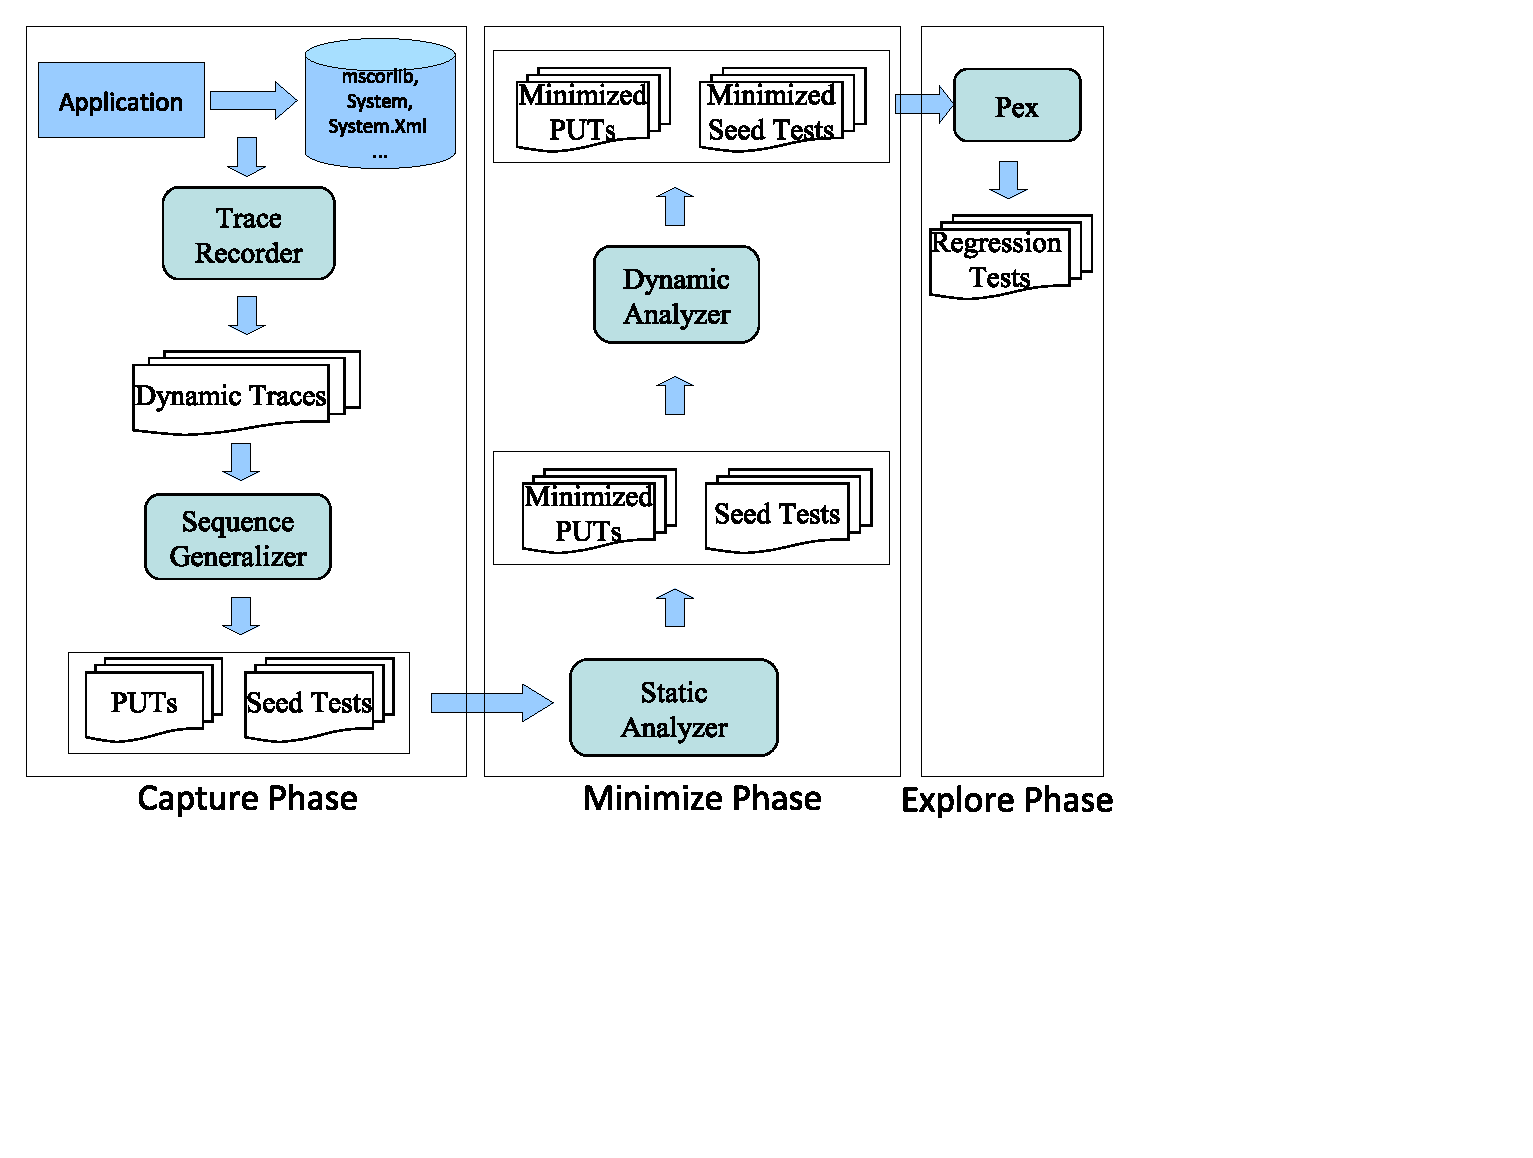
\includegraphics[scale=1,clip]{figure/approach.eps}\vspace*{-3ex}
 \caption{Overview of TeMaAPI}\vspace*{-4ex}
 \label{fig:approach}
\end{figure}
Given a migration tool between Java and C\#, TeMaAPI generates various test cases to reveal different behaviors of the tool's API mapping relations.
Figure~\ref{fig:approach} shows the overview of TeMaAPI.


%-------------------------------------------------------------------
\subsection{Generating client code}
\label{sec:approach:generating}
Given a migration tool, TeMaAPI first extracts its validate mapping relations of APIs. It is challenging to extract such mapping relations directly from a migration tool for two factors: (1) different migration tools may follow different styles to describe API mapping relations. For example, as shown in Section~\ref{sec:introduction}, the API mapping relations of Java2CSharp are described in its mapping files, but the API mapping relations of sharpen are hard-coded in its source files. (2) commercial migration tools typically hide their API mapping relations in binary files. Due to the two factors, TeMaAPI does not extract API mapping relations directly from a migration tool, but chooses to analyze translated code of a migration tool. We choose to use migration tools to translate simple client code instead of existing projects for two considerations: (1) Existing projects typically use quite a small set of APIs, so many API mapping relations may be not covered; (2) a single method of an existing project may use multiple APIs, so it may be difficult to analyze which APIs are not mapped. For the preceding consideration, TeMaAPI chooses to generate client code instead of using existing client code.

TeMaAPI relies on the reflection technique~\cite{maes1987concepts} provided by both Java and C\# to generate client code for translation.

\textbf{Static fields.} Given a public static field \CodeIn{f} of a class \CodeIn{C} whose type is \CodeIn{T}, TeMaAPI generates a getter as follows:
\begin{CodeOut}%\vspace*{-2ex}
\begin{alltt}
 public T TestGet|f.name||no|()\{ return C.f; \}
\end{alltt}
\end{CodeOut}

If \CodeIn{f} is not a constant, TeMaAPI generates a setter as follows:
\begin{CodeOut}%\vspace*{-2ex}
\begin{alltt}
 public void TestSet|f.name||no|(T v)\{ C.f = v; \}
\end{alltt}
\end{CodeOut}

\textbf{Non-static fields.} Given a public non-static field \CodeIn{f} of a class \CodeIn{C} whose type is \CodeIn{T}, TeMaAPI generates a getter for each constructor \CodeIn{C(T1\ p1,\ldots, Tn\ pn)} of \CodeIn{C} as follows:
\begin{CodeOut}%\vspace*{-2ex}
\begin{alltt}
 public T TestGet|f.name||no|(T1\ c1,\ldots, Tn\ cn)\{
    C obj = new C(c1,\ldots, cn);
    return obj.f; \}
\end{alltt}
\end{CodeOut}

If \CodeIn{f} is not a constant, TeMaAPI generates a setter as follows:
\begin{CodeOut}%\vspace*{-2ex}
\begin{alltt}
 public void TestSet|f.name||no|(T1\ c1,\ldots, Tn\ cn)\{
   C obj = new C(c1,\ldots, cn);
   obj.f = v; \}
\end{alltt}
\end{CodeOut}

In the preceding code, ``\CodeIn{|f.name|}'' denotes the name of \CodeIn{f}, and ``\CodeIn{|no|}'' denotes the corresponding number of generated client-code method.

\textbf{Static methods.} Given a public static method \CodeIn{m(T1\ p1,\ldots,Tn\ pn)} of a class \CodeIn{C} whose return type is \CodeIn{Tm}, TeMaAPI generates a client-code method as follows:
\begin{CodeOut}%\vspace*{-2ex}
\begin{alltt}
 public Tm Test|m.name||no|(T1\ m1,\ldots, Tn\ mn)\{
   return C.m(m1,\ldots, mn); \}
\end{alltt}
\end{CodeOut}

\textbf{Non-static methods.} Given a public non-static method \CodeIn{m(T1\ p1,\ldots,Tn\ pn)} of a class \CodeIn{C} whose return type is \CodeIn{Tm}, TeMaAPI generates a client-code method for each constructor \CodeIn{C(Tv\ pv,\ldots, Tt\ pt)} of \CodeIn{C} as follows:
\begin{CodeOut}%\vspace*{-2ex}
\begin{alltt}
 public Tm Test|m.name||no|(T1\ m1,\ldots, Tn\ mn,
                            Tv cv, \ldots, Tt ct)\{
   C obj = new C(cv,\ldots, ct);
   return obj.m(m1,\ldots, mn); \}
\end{alltt}
\end{CodeOut}

In the preceding code, ``\CodeIn{|m.name|}'' denotes the name of \CodeIn{m(T1\ p1,\ldots,Tn\ pn)}.

TeMaAPI ignores generic methods for simplicity, and organizes all generated client code methods by the corresponding class $C$. For a migration tool that translates from Java to C\#, TeMaAPI generates client code in Java as shown by the solid line of Figure~\ref{fig:approach}, and for a migration tool that translates from C\# to Java, TeMaAPI generates client code in C\# as shown by the dotted line of Figure~\ref{fig:approach}. When TeMaAPI generates client code in C\#, it ignores \CodeIn{unsafe} and \CodeIn{delegate} methods and methods whose parameters are marked as \CodeIn{our} or \CodeIn{ref}. Java does not have corresponding keywords, so there are typically no mapped methods in Java for these C\# methods. After TeMaAPI generate client-code methods, we translate them using a migration tool under experiments.


%-----------------------------------------------------------------
\subsection{Analyzing Generated Methods}
\label{sec:approach:analyzing}
Translated code typically contain many compilation errors since a migration tool typically cannot cover mapping relations of all APIs. TeMaAPI then analyzes translated code for validate API mapping relations of the migration tool. To achieve this, TeMaAPI first remove all translated methods with compilation errors. For translated methods in Java, TeMaAPI implements a Eclipse plug-in that uses on Eclipse JDT compiler\footnote{\url{http://www.eclipse.org/jdt/}} for the list of compilation errors. For translated methods in C\#, TeMaAPI implements a Visual Studio.Net add-in to retrieve the list of compilation errors from the error-list view of Visual Studio.Net. Both Eclipse JDT compiler and Visual Studio.Net cannot list all methods with compilation errors in a single build. After each iteration of removing methods, TeMaAPI re-build these methods until it removes all methods with compilation errors.

After methods with compilation errors are removed, TeMaAPI compares generated code with translated code for the validate API mapping relations of a migration tool. Based on translated code and validate API mapping, TeMaAPI removes generated methods whose corresponding translated methods have compilation errors. We refer to those removing client-code methods as safe methods.

%-----------------------------------------------------------
\subsection{Finding Different Behaviors}
\label{sec:approach:behavior}
In the final step, TeMaAPI generates test cases to detect different behaviors of API mapping relations. An alternative approach is to use existing test cases in two languages. For example, lucene\footnote{\url{http://lucene.apache.org}} has both a Java version and a C\# version. It is feasible to use these test cases to reveal some different behaviors, but such test cases typically cover only a small set of APIs. Some test suites such as Java Compatibility Kit (JCK)\footnote{\url{http://jck.dev.java.net}} cover most APIs of a language. However, translating such a test suite from one language into another language may introduce many compilation errors and defects. A test method may use many APIs, so even if the API under test can be translated correctly, the test method cannot be translated correctly since other APIs are not mapped. As a result, we choose to translating existing test suites as a supplement of our approach.

\subsubsection{Generating Test Cases}
\label{sec:approach:behavior:generating}
For each safe method in Java, we use Randoop~\cite{pacheco2007feedback} to generate its test cases. For each safe method in C\#, we use Pex~\cite{tillmann2008pex} to generate its test cases. TeMaAPI then executes generated test cases, and records the inputs, the output, and the thrown exception of each test case as a file.

Based on the file, TeMaAPI generates Junit\footnote{\url{http://www.junit.org/}} or Nunit\footnote{\url{http://www.nunit.org/}} test cases to ensure each mapped API produce the same output give the same inputs. For example, Pex generates a test case whose input is \CodeIn{m0 = false} for the \CodeIn{TestvalueOf57} method in C\# as shown in Section~\ref{sec:example}, and after executing the output of the test case is ``False''. Based on the input and the output of this test case, TeMaAPI generates a Junit test case as follows:

\begin{CodeOut}%\vspace*{-2ex}
\begin{alltt}
 @Test
 public void testvalueOf64zhh0()\{
   sketch.Test_java_lang_String obj =
                       new sketch.Test_java_lang_String();
   boolean m0 = false;
   Assert.assertEquals("False", obj.testvalueOf64(m0));\}
\end{alltt}
\end{CodeOut}

This Junit test case fails since the preceding \CodeIn{testvalueOf64zhh} method produces ``false'' instead of ``False''. From this failed Junit test case, TeMaAPI detects that the \CodeIn{java.lang.String.valueOf (Object)} method in Java has different behaviors with its mapped C\# methods if inputs are boolean values.

In some cases, executing a test case does not produce outputs but exceptions. For example, Pex also generates a test case whose input is \CodeIn{m0 = null} for the \CodeIn{TestvalueOf57} method in C\# as shown in Section~\ref{sec:example}, after executing it throws \CodeIn{NullReferenceException}. TeMaAPI finds that the \CodeIn{NullPointerException} class in C\# is mapped to the \CodeIn{NullPointerException} class in Java in the validate API mapping relations, and generates a Junit test case based on the preceding mapping relation and input as follows:

\begin{CodeOut}%\vspace*{-2ex}
\begin{alltt}
 @Test
 public void testvalueOf64zhh3()\{
   try\{
     sketch.Test_java_lang_String obj =
                       new sketch.Test_java_lang_String();
     boolean m0 = null;
     obj.testvalueOf64(m0);\}
   \}catch(java.lang.NullPointerException e)\{
       Assert.assertTrue(true);
       return;
   \}
   Assert.assertTrue(false);\}
\end{alltt}
\end{CodeOut}

This Junit test case also fails since given a null input, the preceding \CodeIn{testvalueOf64} method does not throw any exceptions. From this failed Junit test case, TeMaAPI detects that the \CodeIn{java.lang. String.valueOf(Object)} method in Java has different behaviors with its mapped C\# methods if inputs are null pointers.

\subsubsection{Translating Existing Test Cases}
\label{sec:approach:behavior:jck}

Each generated client-code method uses only one fields or methods provided by API libraries, and may lose some complicated behaviors even if test cases satisfy the round-trip criterion. To test those complicated behaviors, we introduce JCK that covers many complicated behaviors of Java APIs. JCK is a test suite provided by Sun to ensure compatibility of Java platforms, and it covers most standard APIs of J2SE. However, JCK implements many internal classes to collect the results of executed test cases. If a migration tool cannot correctly translate one of these classes, all translated test cases may have compilation errors or defects. In addition, JCK is released under read-only source license\footnote{\url{http://tinyurl.com/33x9fo6}}, so many such internal classes are not shipped and it has many compilation errors. To increase the chance of migrating JCK, TeMaAPI first replaces those internal classes with the classes of Junit. For example, one test method for \CodeIn{java.io.File.delete()} in JCK is as follows:

\begin{CodeOut}%\vspace*{-2ex}
\begin{alltt}
  public Status File0037()\{
    String testCaseID = "File0037";
    ...
    FileRT method = new FileRT(testCaseID) \{
     public Status run() \{
       File f = null;
       f = new File(workdir, testCaseID);
       ...
       if (f.delete()) \{ // Try to delete
         if (!f.exists()) \{ // Does it exist?
           return Status.passed("OKAY");
         \}else\{
            return Status.failed(...);
         \}
       else\{
           return Status.failed(...);
       \}
    \}
     return AllPermissionSM.testRun(...);
  \}
\end{alltt}
\end{CodeOut}

After the preceding three steps, TeMaAPI further replaces the statement starts with \CodeIn{FileRT} with the body of the \CodeIn{run} method, and removes the last statement. The translated code is as follows:

\begin{CodeOut}%\vspace*{-2ex}
\begin{alltt}
  public void File0037()\{
    String testCaseID = "File0037";
    ...
    File f = null;
    f = new File(workdir, testCaseID);
    ...
    if (f.delete()) \{ // Try to delete
      if (!f.exists()) \{ // Does it exist?
        Assert.assertTrue(true);
        return;
     \}else\{
        Assert.fail();
        return;
     \}
   else\{
       Assert.fail();
       return;
   \}
  \}
\end{alltt}
\end{CodeOut}

Compared with the original test method in JCK, the translated method does not use the three internal classes: \CodeIn{Status}, \CodeIn{FileRT}, and \CodeIn{AllPermissionSM}. 

After the preceding process, for a migration tool, TeMaAPI further removes methods that use any APIs outside its defined mapping relations. The remaining methods can be translated from Java to other languages since it does not use any APIs outside of the migration tool.



\section{Design}
\label{design}

The objective of this project is to automatically generate a method-call sequence for a given desired object state. Figure~\ref{fig:mut} shows a method under test of the class \CodeIn{UndirectedDepthFirstSearchAlgorithm} of the QuickGraph library. To cover Statement 9 in the method under test, the field \CodeIn{VisitedGraph} should include edges. Currently, without any assistance Pex cannot cover Statement 9 as it is non-trivial to generate a graph instance with vertices and edges.

\begin{figure}[t]
\begin{CodeOut}
\begin{alltt}
00:public void Compute(IVertex s) \{
01:\hspace*{0.2in}// init vertices
02:\hspace*{0.2in}foreach(IVertex u in VisitedGraph.Vertices) \{
03:\hspace*{0.3in}Colors[u]=GraphColor.White;
04:\hspace*{0.3in}if (InitializeVertex != null)
05:\hspace*{0.4in}InitializeVertex(this, new VertexEventArgs(u));
06:\hspace*{0.2in}\}
07:\hspace*{0.2in}//init edges
08:\hspace*{0.2in}foreach(IEdge e in VisitedGraph.Edges) \{
09:\hspace*{0.3in}EdgeColors[e]=GraphColor.White;
10:\hspace*{0.2in}\}
11:\hspace*{0.2in}// use start vertex
12:\hspace*{0.2in}if (s != null) \{
13:\hspace*{0.3in}if (StartVertex != null)
14:\hspace*{0.4in}StartVertex(this,new VertexEventArgs(s));
15:\hspace*{0.3in}Visit(s);
16:\hspace*{0.2in}\}
17:\hspace*{0.2in}// visit vertices
18:\hspace*{0.2in}foreach(IVertex v in VisitedGraph.Vertices) \{
19:\hspace*{0.3in}if (Colors[v] == GraphColor.White) \{
20:\hspace*{0.4in}if (StartVertex != null)
21:\hspace*{0.5in}StartVertex(this,new VertexEventArgs(v));
22:\hspace*{0.3in}Visit(v);
23:\hspace*{0.2in}\}
24:\hspace*{0.2in}\}
25:\}
\end{alltt}
\end{CodeOut}
\Caption{\label{fig:mut} A method under test from the QuickGraph library.}
\end{figure}

\subsection{Capture the desired object state}

The first step of our approach is to capture the desired object state (with respect to fields in object types) from the branch that is not covered in the method under test. Figure~\ref{fig:condition} shows the object state captured by the current SeqEx approach. The field that is actually responsible for not able to cover the branch is \CodeIn{ArrayList.\_size}. First, it has to be identified that the uncovered branch (Statement 9) in the method under test is due to the desired condition shown in Figure~\ref{fig:condition}. We can use the approach Covana (developed by Xusheng) to address this issue. We next explain how to generate a method-call sequence for achieving the desired object state.

\begin{figure*}[t]
\begin{CodeOut}
\begin{alltt}
Code location: System.Collections.ArrayList+ArrayListEnumeratorSimple.MoveNext at 0x003e
field: System.Collections.ArrayList._size
field: System.Collections.CollectionBase.list
field: QuickGraph.Representations.AdjacencyGraph.m_Edges
field: QuickGraph.Algorithms.Search.UndirectedDepthFirstSearchAlgorithm.m_VisitedGraph
path condition term: 
UndirectedDepthFirstSearchAlgorithm s7 = new;
AdjacencyGraph s6
   = target == s7 ? g_iVertexAndEdgeListGraph : (AdjacencyGraph)(target.m_VisitedGraph);
AdjacencyGraph s5 = s6;
EdgeCollection s8 = new;
EdgeCollection s4 = s5 == (AdjacencyGraph)s7 ? s8 : s5.m_Edges;
EdgeCollection s3 = s4;
EdgeCollection s2 = s3 == s8 ? s8 : (EdgeCollection)(((CollectionBase)s3).list);
EdgeCollection s1 = s2;
int s0 = s1 == s8 ? 0 : ((ArrayList)s1).\_size;
return -1 < -1 + s0;
\end{alltt}
\end{CodeOut}
\Caption{\label{fig:condition} Desired object state captured by the current SeqEx approach.}
\end{figure*}

\subsection{Identifying methods of interest}

Our approach will next identify the methods that modify the fields captured in the desired object state. To address this issue, we need several types of information, which can be gathered either dynamically or statically. In our approach, We plan to use a combination of dynamic and static analyses for achieving this purpose. The advantage of using dynamic analysis is that captured information is precise. However, only a limited information can be captured as dynamic analysis requires the relevant portions of the code to be executed. On the other hand, the information captured using static analysis is imprecise due to its conservative nature.

In our approach, we need to capture the following types of information:

\begin{itemize}
\item Modified Fields: Includes information of which fields are modified by different methods of classes in the application under analysis. Useful for detecting the methods of interest.
\item Read Fields: Includes information of which fields are read by different methods. This is useful to detect dependencies among methods.
\item Caller/Callee Methods: Includes information of methods called by different methods.
\end{itemize}

Using \emph{Modified Fields}, it is possible to identify the methods that affect the \CodeIn{\_size} field as \CodeIn{Add} and \CodeIn{Remove} methods of the \CodeIn{ArrayList} class. In total, there are $0$ methods that modify the \CodeIn{\_size} field. It is required to identify which method to choose for achieving desired object state. We plan to use two techniques to precisely choose the method to achieve desired object state.

The first technique is to prune out the methods of the \CodeIn{ArrayList} class that are not invoked by its callers in the application under analysis. 
However, these methods cannot be directly invoked as the instance of the \CodeIn{ArrayList} class is not visible outside. Therefore, it is required to identify the object (which is visible) and also the method of the instance, which can be invoked. We plan to use the \emph{Called/Callee Methods} information to address this issue. More specifically, we construct a directed graph as shown in Figure~\ref{}. The objective of our algorithm is to identify an object whose level is as minimum as possible and an associated method of the object that 

%%%%%%%%%%%%%%%%%%%%%%%%%%%%%%%%%%%%%%%%%%%%%%%%%%%%%%%%%%%%%%%%%%%%%%%%%%%%%%%%%%%%%%%%%%%%%%%%%%%%%%%%%%%%%%%%
% PREVIOUS DESIGN BASED ON CONSTRAINT SOLVING

%The objective of this project is to automatically generate a method-call sequence for a given desired object state. Figure~\ref{fig:simplestack} shows a simple stack implementation. Figure~\ref{fig:mut} shows a method under test using the \CodeIn{SimpleStack}. To cover the \CodeIn{true} branch of the \CodeIn{if} method, the desired object state is to have more than five elements in the stack. The desired method-call sequence for achieving this desired object state is to create an instance of \CodeIn{SimpleStack} and invoke the \CodeIn{Push} method for six or more times. We next explain our proposed approach in detail.
%
%\begin{figure}[t]
%\begin{CodeOut}
%\begin{alltt}
%public class SimpleStack \{
%\hspace*{0.2in}int count;
%\hspace*{0.2in}int[] elements;
%\hspace*{0.2in}int currentPosition;
%\hspace*{0.2in}public SimpleStack() \{
%\hspace*{0.3in}elements = new int[20];
%\hspace*{0.3in}currentPosition = 0;
%\hspace*{0.3in}count = 0;
%\hspace*{0.2in}\}
%
%\hspace*{0.2in}public void Push(int i) \{
%\hspace*{0.3in}if (currentPosition >= 20)
%\hspace*{0.4in}throw new Exception("Stack full");
%\hspace*{0.3in}elements[currentPosition++] = i;
%\hspace*{0.3in}count++;
%\hspace*{0.2in}\}
%
%\hspace*{0.2in}public int Pop() \{
%\hspace*{0.3in}if (currentPosition == 0)
%\hspace*{0.4in}throw new Exception("Stack empty");
%\hspace*{0.3in}count--;
%\hspace*{0.3in}return elements[--currentPosition];
%\hspace*{0.2in}\}
%
%\hspace*{0.2in}public int Size() \{
%\hspace*{0.3in}return count;
%\hspace*{0.2in}\}
%\}
%\end{alltt}
%\end{CodeOut}
%\Caption{\label{fig:simplestack} Simple Stack Implementation.}
%\end{figure}
%
%\begin{figure}[t]
%\begin{CodeOut}
%\begin{alltt}
%\hspace*{0.2in}public void MUT(SimpleStack st) \{
%\hspace*{0.3in}if (st.Size() > 5) \{
%\hspace*{0.4in}...
%\hspace*{0.2in}\}
%\}
%\end{alltt}
%\end{CodeOut}\vspace*{-3ex}
%\Caption{\label{fig:mut} Method under test.}\vspace*{-3ex}
%\end{figure}
%
%\subsection{Capture desired object state}
%
%When a particular branch in the code under test is not covered, our approach will precisely capture the desired object state (with respect to fields in object types) from the branch that is not covered in the code under test. For example, in our method under test, the desired object state should be the field \CodeIn{count} of \CodeIn{SimpleStack} should be greater than five. 
%
%The desired object state can be more complex and often lead to another desired object state. For example, consider another class under test \CodeIn{InternalFields} (Figure~\ref{fig:iftest}) and MUT (Figure~\ref{fig:iftest}). In this scenario, the desired state is the field \CodeIn{localState} should be \CodeIn{true}. However, the local state is set to \CodeIn{true} in the method \CodeIn{SetLocalState} (a \CodeIn{private} method) when other fields are in certain desired object state such as \CodeIn{member1 == 5}, \CodeIn{member2 == 3}, and \CodeIn{member3 $>$ 2}. This example illustrates a chaining scenario while capturing the desired object state. In particular, addressing one desired object state can lead to multiple desired states that need to be further addressed.
%
%\begin{figure}[t]
%\begin{CodeOut}
%\begin{alltt}
%\emph{InternalFields CUT}
%public class InternalFields \{
%\hspace*{0.2in}private int member1, member2, member3;
%\hspace*{0.2in}private bool localState;
%\hspace*{0.2in}public bool InternalState \{
%\hspace*{0.3in}get \{
%\hspace*{0.4in}return localState;
%\hspace*{0.3in}\}
%\hspace*{0.2in}\}
%\hspace*{0.2in}private void SetLocalState() \{
%\hspace*{0.3in}if (member1 == 5 && member2 == 3 && member3 > 2)
%\hspace*{0.4in}localState = true;
%\hspace*{0.2in}\}
%\hspace*{0.2in}public void IncrM1() \{
%\hspace*{0.3in}member1++;
%\hspace*{0.3in}SetLocalState();
%\hspace*{0.2in}\}
%\hspace*{0.2in}public void IncrM2AndDecrM1() \{
%\hspace*{0.3in}member2++;
%\hspace*{0.3in}member1--;
%\hspace*{0.3in}SetLocalState();
%\hspace*{0.2in}\}
%\hspace*{0.2in}public void IncrM3AndDecrM1() \{
%\hspace*{0.3in}member3++;
%\hspace*{0.3in}member1--;
%\hspace*{0.3in}SetLocalState();
%\hspace*{0.2in}\}   
%\}
%\emph{Method Under Test}
%public void FieldCheck(InternalFields ifd) \{
%\hspace*{0.2in}if (ifd.InternalState) \{
%\hspace*{0.3in}...
%\hspace*{0.2in}\}
%\}
%\end{alltt}
%\end{CodeOut}
%\Caption{\label{fig:iftest} InternalFields Class and a method under test based on this class.}
%\end{figure}
%
%\subsection{Identifying methods of interest}
%
%Our approach will next identify the methods of the class under test that modify the fields captured in the desired object state. For example, in the case of \CodeIn{SimpleStack}, our approach will identify that the \CodeIn{count} field is modified by the methods \CodeIn{Push} and \CodeIn{Pop}. Similarly, in the case of \CodeIn{InternalFields}, our approach will identify that \CodeIn{member1} is modified by \CodeIn{IncrM1}, \CodeIn{IncrM2AndDecrM1}, and \CodeIn{IncrM3AndDecrM1}. Our approach will next identify how many times each method has to be invoked. 
%
%To address this issue, our approach will first generate conditional terms (suitable for solving via a constraint solver) that represent the desired object state in terms of method calls. For example, the field \CodeIn{count} is increased by the \CodeIn{Push} method and is decreased by the \CodeIn{Pop} method. Lets consider that ``X'' represents the number of times the \CodeIn{Push} method has to be called and ``Y'' represents the number of times the \CodeIn{Pop} method has to be called. The equation for the \CodeIn{count} field to achieve desired object state is ``X - Y $>$ 5''. There can be multiple equations based on the desired object state.
%
%For the \CodeIn{InternalFields} class, to achieve the desirable object, the method \CodeIn{SetLocalState} has to be invoked once. Therefore, the terms for achieving this state are ``S == 1'', where S represents the number of times the method \CodeIn{SetLocalState} has to be invoked. However, invoking this method simply does not achieve the desired object state as it requires another state to be achieved for covering the \CodeIn{true} branch of the \CodeIn{SetLocalState} method. This chaining of desired states  can be identified by executing the current sequence and by discovering new branches that are not covered. Our approach will next construct more terms that represent the new state to be achieved. Consider that ``X'' represents the number of times \CodeIn{IncrM1} has to be invoked, ``Y'' represents the number of times \CodeIn{IncrM2AndDecrM1} has to be invoked, and ``Z'' represents the number of times \CodeIn{IncrM3AndDecrM1} has to be invoked. The terms for achieving desired object state are as follows:
%
%\begin{center}
%\begin{CodeOut}
%\begin{alltt}
%S == 1
%X - Y - Z == 5
%Y == 3
%Z > 2
%\end{alltt}
%\end{CodeOut}
%\end{center}
%
%Using constraint solver, these terms can be solved to get concrete values for fields S, X, Y, and Z. These concrete values represent the number of times the associated method calls has to be invoked to achieve desired object states. In our current example, a constraint solver can return values for S, X, Y, and Z as 1, 11, 3, and 3, respectively. Based on this information, it can be inferred that an example desired method-call sequence can be as follows:
%
%\begin{CodeOut}
%\begin{alltt}
%InternalFields internalFields = new InternalFields();
%for(int c1 = 0; c1 < 11; c1++)
%\hspace*{0.3in}internalFields.IncrM1();
%for (int c2 = 0; c2 < 3; c2++)
%\hspace*{0.3in}internalFields.IncrM2AndDecrM1();
%for (int c3 = 0; c3 < 3; c3++)
%\hspace*{0.3in}internalFields.IncrM3AndDecrM1();            
%return internalFields;
%\end{alltt}
%\end{CodeOut}
%
%\subsection{Getting an instance of class under test}
%
%Existing approaches such as Prospector~\cite{prospector:jungloid} or JCrasher~\cite{csallner:jcrasher} can be used to identify how to get an instance of the desired class under test. These approaches constructs a graph, referred to as signature graph, from the signatures of APIs. This signature graph helps to get an instance of the target class under test. Although these approaches help in getting target class under test, these approaches do not help in generating desired object state for the class under test. More specifically, their signature graphs often do not include the state-modifying methods of the class under test.
%
%\subsection{Inferring specification of class under test}
%
%It is often not sufficient to identify what are the methods of interest, since there can be several dependencies among methods. Due to those dependencies, it is often possible that the generated method-call sequences are not valid (i.e., they may result in compilation errors or throw run-time exceptions). For example, we also need information on the sequence of how to invoke the identified methods under test. Furthermore, it is required to capture any additional methods that have to be invoked before invoking the identified methods under test. For example, consider a variant of the class \CodeIn{InternalFields} shown in Figure~\ref{fig:iftest1}, which is more simpler than the original class. It is easy to identify that the desired object state can be achieved by invoking the method \CodeIn{IncrM1} five times. However, the method \CodeIn{IncrM2} should also be called five times along with the method \CodeIn{IncrM1}. Inferring specifications for the class under test can help address these issues. For example, a simple specification in terms of the finite automaton for the \CodeIn{MultiMethodsInLoop} is shown in Figure~\ref{fig:loopfsa}. The specification describes several aspects such as \CodeIn{IncrM2} should be called before \CodeIn{IncrM1}. The specification also shows that \CodeIn{IncrM2} should be called after \CodeIn{IncrM1} before invoking \CodeIn{IncrM1} again.
%
%\begin{figure}[t]
%\begin{CodeOut}
%\begin{alltt}
%public class MultiMethodsInLoop \{
%\hspace*{0.2in}private int member1, member2, member3;
%\hspace*{0.2in}private bool localState;
%\hspace*{0.2in}bool m1set = true, m2set = false;
%        
%\hspace*{0.2in}public bool InternalState \{
%\hspace*{0.3in}get \{
%\hspace*{0.4in}return localState;
%\hspace*{0.3in}\}
%\hspace*{0.2in}\}
%
%\hspace*{0.2in}private void SetLocalState() \{
%\hspace*{0.3in}if (member1 == 5)
%\hspace*{0.4in}localState = true;
%\hspace*{0.2in}\}
%
%\hspace*{0.2in}public void IncrM1() \{
%\hspace*{0.3in}if (!m2set)
%\hspace*{0.4in}throw new Exception("Member2 is not set properly");
%\hspace*{0.3in}member1++;
%\hspace*{0.3in}SetLocalState();
%\hspace*{0.3in}m1set = true;
%\hspace*{0.3in}m2set = false;
%\hspace*{0.2in}\}
%
%\hspace*{0.2in}public void IncrM2() \{
%\hspace*{0.3in}if (!m1set)
%\hspace*{0.4in}throw new Exception("Member1 is not set properly");
%\hspace*{0.3in}m2set = true;
%\hspace*{0.3in}m1set = false;
%\hspace*{0.2in}\}
%\}
%\end{alltt}
%\end{CodeOut}
%\Caption{\label{fig:iftest1} \CodeIn{MultiMethodsInLoop} Class, which is a variant of \CodeIn{InternalFields}.}
%\end{figure}
%
%\begin{figure}[t]
%\centering
%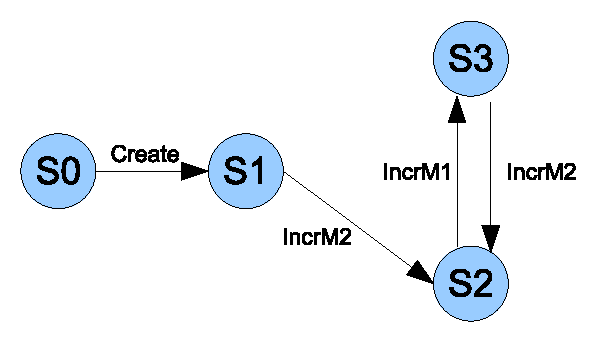
\includegraphics[scale=0.60,clip]{figs/MultiMethodsLoopFsa1.eps}
%\caption{\label{fig:loopfsa}Finite automaton for MultiMethodsLoop class.}
%\end{figure}
%
%These specifications can be inferred either by applying mining approaches on existing code bases~\cite{thummalapenta09:mseqgen} or from the implementation of the class under test~\cite{whaley02:interface}. Inferring complete specifications for all methods of the class under test can itself be a challenging problem that need to be addressed. For example, the approaches that infer specifications from the implementation are not scalable in practice. On the other hand, the approaches that infer specifications using mining approaches may not be able to infer specification for a method if that method is not used by any existing code bases. Therefore, a synergy of these two approaches can help effectively infer specifications.
%
%\subsection{Using specification for sequence generation}
%
%Our approach will next generate sequences that achieve desirable object states based on the inferred specification and the methods of interest. As we already know the methods of interest, the automaton representing can be pruned by not covering those paths that do not include our methods of interest. Next, our approach will explore this automaton to achieve the desired object state by visiting each method as desired number of times.
%
%\subsection{Open Problems}
%
%The current design is based on an assumption that it is possible to infer method summaries, which describe how methods of a class under test are modifying its fields. However, in case of classes from external libraries, it may not be possible to infer method summaries. 
\section{Preliminary Evaluation}
\label{sec:prelims}

We next present the preliminary results gathered by minually using the information from our approach. We use examples
from four real-world applications to show the preliminary results of our feasibility study. Column ``Before'' shows the block coverage achieved 
by Pex without the assistance from our approach. Column ``After'' shows the block coverage achieved after the assistance from the approach.
The results show that Pex achieves better code coverages with the assistance of our approach.

\begin{table*}[t]
\begin{SmallOut}
\begin{CodeOut}
\begin{center}
\centering \caption {\label{tab:results} Preliminary results of manual analysis.}
\begin {tabular} {|l|c|c|c|}
\hline
Subject & Class Under Test & Before & After\\
\hline
\hline QuickGraph & UndirectedDepthFirstSearchAlgorithm & 21/81 (28.40\%) & 81/130 (62.31\%)\\
\hline 						& TopologicalSortAlgorithm 						& 13/20 (65.00\%) & 16/23  (69.57\%)\\
\hline						&	DepthFirstSearchAlgorithm						& 25/56 (44.64\%) & 66/105 (62.00\%)\\
\hline NUnit		  & MemorySettingsStorage								& 16/31 (51.00\%) & 24/33  (72.73\%)\\
\hline						& SettingsStorage											& 5/28  (17.86\%) & 15/28  (53.57\%)\\
\hline NHibernate & Table																& 41/44 (93.18\%) & 43/44  (97.75\%)\\
\hline						& ForeignKey 													& 30/43 (69.77\%) & 58/61  (95.08\%)\\
\hline DSA			  & SinglyLinkedList									  & 8/28  (28.57\%) & 27/38  (71.05\%)\\
\hline
\end{tabular}
\end{center}
\end{CodeOut}
\end{SmallOut}\vspace*{-6ex}
\end{table*}





\bibliographystyle{abbrv}
\bibliography{Seqex}

\end{document}
